%we have some fixed parameters such as light control on or off. Mimics intersection lights.\\
%Whether simulated vehicles are able to turn or not.\\
%We have different max speeds - 60 or 40 km per hour approach. This translates to lower speeds %during turns (roughly half).\\

%tests are different combinations of above parameters. And results are measured in collisions, cars spawned, cars reaching destination, and time before deadlock.\\
%Deadlock is the situation where cars have been stuck for a period of time in the `intersection zone' without entering or leaving.

%To test the implementation of our system we ran some simulations 
To compare performances of the system over different paradigms and with different parameters, we ran
multiple experimental simulations.
The parameters that we changed over the different tests are from three classes: the paradigm, the speed of the cars, and the complexity.

For paradigm it is meant the use of  a traffic light regulated intersection versus a pure reactive approach.
As for complexity, we can increase it by allowing the cars to turn in order to reach any destination, or we can use a simpler system where cars can only go straight.

The car speed is changed over three base cases: slow ( 30 km/h), medium (40 km/h) and fast (60 km/h).
It is worth mentioning that the advised speed when turning the car in 90 degrees turns inside urban areas is around or below 30 km/h. %todo find reference

When simulating with traffic lights enabled, we test two intervals of time that regulate the duration of the green light.
We have an interval window of approximately 1 minute, that reflects a realistic scenario according to our observation of real life intersections.
We also test a much shorter window of 20 seconds, that should improve performance under the assumptions that:
\begin{enumerate}
\item autonomous vehicles can react faster than human drivers, so they can start moving immediately after the traffic light turns green compared to human drivers that could be slow or distracted;
\item shorter windows of time allow the traffic to be managed evenly, since traffic is evenly distributed between the different directions.
\end{enumerate}

\subsection{Experimental results}

We measure performance of the systems mainly in terms of throughput, namely the amount of cars that get through the intersection per minute.
However, we also account for other factors, like the amount of collisions, the amount of deadlock situations, the time at which these occur and the frequency of these events.

A deadlock is the condition in which cars have been stuck in the intersection zone with no one entering or leaving for a period of time (about 10 seconds).

To test the implementation of our system we also account for information such as the number of cars spawned, number of cars "lost" (not reaching the correct destination) and the number of cars present in the intersection zone at the occurrence of a deadlock or collision.

\subsubsection{Throughput}
The graphs in figure \ref{fig:throughput} show the different throughputs of the system running with different factors.

\begin{figure}
\centering
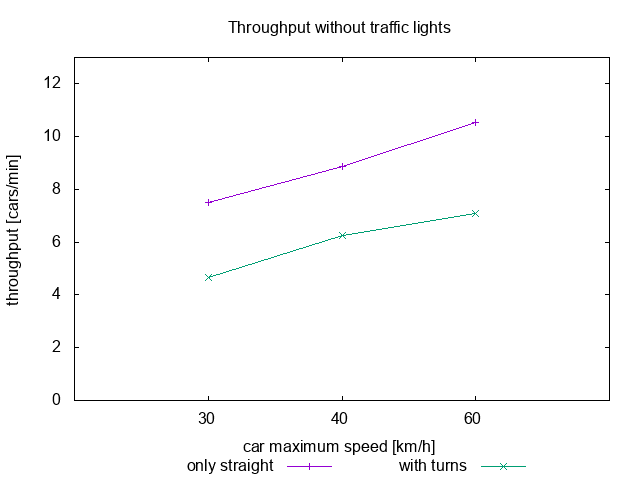
\includegraphics[scale=0.5]{img/plot_throughmin_notl}
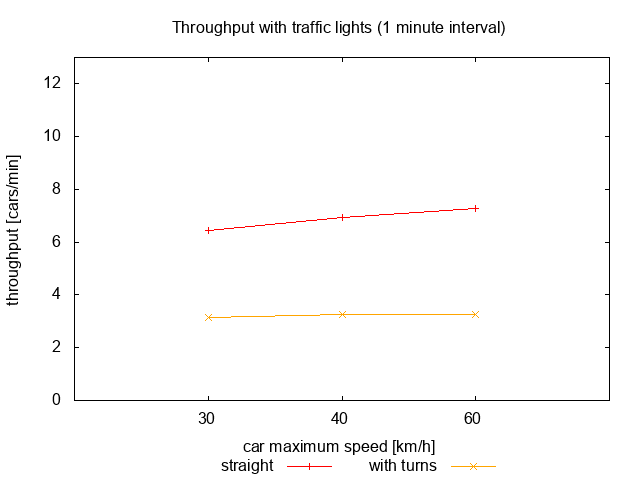
\includegraphics[scale=0.5]{img/plot_throughmin_tl}
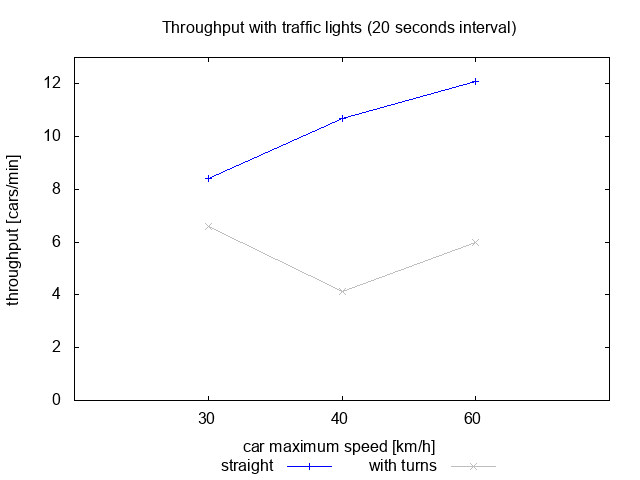
\includegraphics[scale=0.5]{img/plot_throughmin_tl20}
\caption{Throughputs in comparison}
\label{fig:throughput}
\end{figure}
